Nachdem nun die Spezifikationen und Protokolle im einzelnen vorgestellt wurden, muss die E-Mail als Gesamtsystem betrachtet werden. Dazu wird nachfolgend untersucht, wie die Komponenten zusammengeführt werden, miteinander kommunizieren und wie eine Server-Konfiguration grob in der Praxis aussieht.

Auf der untersten Ebene befindet sich der \QuoteM{Mail User Agent}, kurz MUA. Er bezeichnet ein gewöhnliches E-Mail Programm, mit dem E-Mails gelesen, verfasst, empfangen und gesendet werden können. Beispiele hierfür sind Programme wie etwa \QuoteM{Mozilla Thunderbird}
oder \QuoteM{Outlook Express}.
Dies ist die Stelle, an der der Benutzer dem System Input gibt. Ein solches Programm muss in der Lage sein, mit allen Protokollen und Spezifikationen umzugehen. Für den Versand ist das beispielsweise IMF und SMTP, für das Empfangen und Manipulieren von E-Mails beispielsweise POP3 oder IMAP4.
Dies findet alles beim Benutzer statt, ist also clientseitig.

Auf der nächsten Ebene befindet sich der sogenannte E-Mail Server. Allerdings besteht dieser aus mehreren Komponenten. Mehrere E-Mail Server können sehr unterschiedliche Funktionalitäten bereitstellen, obwohl sie alle das SMTP Protokoll implementiert haben. Wenn der Benutzer über einen MUA eine E-Mail verschicken will, so sendet er diese an einen sogenannten \QuoteM{Mail Submission Agent} häufig an Port 587 \QuoteIndirect{rfc6409}{S. 6}, kurz MSA. Über diesen wird die initial erstellte E-Mail empfangen und gelangt so in den Zustellungsmechanismus.

Nachfolgend kann die E-Mail nun, abhängig vom Zustellungsmechanismus, über mehrere sogenannte \QuoteM{Mail Transfer Agents}, kurz MTA, weitergeleitet werden. Für jede Weiterleitung wird der E-Mail ein Headerfeld \verb#Received:# hinzugefügt, über welches der Weg, den die E-Mail über mehrere MTAs genommen hat, nachvollzogen werden kann. Der MTA ist die zentrale Einheit der E-Mail Zustellung, da er E-Mails versendet und empfängt.

Gelangt die E-Mail zum E-Mail Server des Empfängers, so wird der sogenannte \QuoteM{Mail Delivery Agent}, kurz MDA, aktiv. Dieser hat die Aufgabe, die E-Mail dem korrekten Benutzerkonto zuzuordnen, da ein E-Mail Server für gewöhnlich mehrere Benutzerkonten bereitstellt.

Auf der letzten Ebene befindet sich erneut ein MUA, und zwar in diesem Fall der des Empfängers, der nun über einen in seinem E-Mail Server integrierten POP3 oder IMAP4 Dienst die E-Mail abrufen kann.

Das bedeutet, dass ein E-Mail Server verschiedene Formen haben kann, z.B.:
\begin{itemize}
\item ein MTA, ein MSA, ein MDA und ein IMAP4 und POP3 Server, gewissermaßen als vollständige Lösung
\item nur ein MSA und MTA, der empfangene E-Mails an einen vordefinierten E-Mail Server weiterleitet, gewissermaßen als SMTP Gateway
\item nur ein MTA, z.B. als offenes oder internes Relay
\end{itemize}

\begin{figure}[htb]
	%\Centerfloat
	\centering
	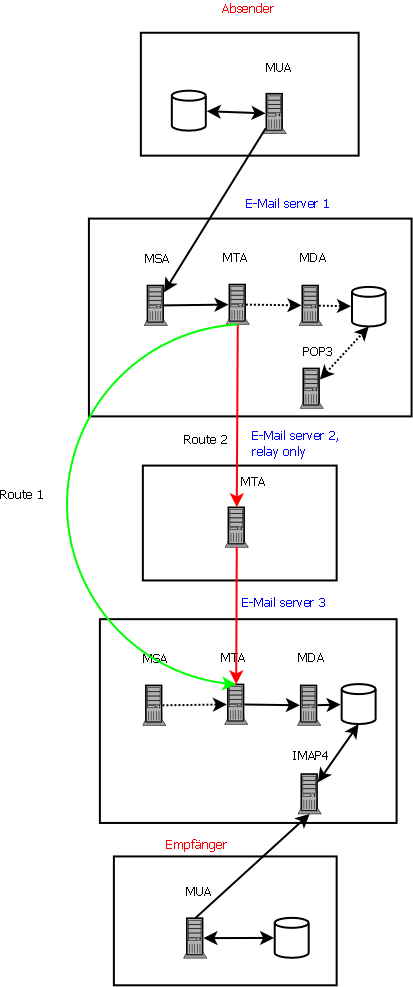
\includegraphics[scale=0.5]{Content/Intro/Protokolle/emailg.png}
	\caption{E-Mail als Gesamtsystem}
	\label{fig:emailg}
\end{figure}

\vfill
\clearpage

Die \autoref{fig:emailg} zeigt schematisch das Zusammenspiel der Komponenten:
Der ursprüngliche Absender erstellt über seinen MUA die E-Mail. Der MUA kontaktiert den MSA des \QuoteM{E-Mail Server 1} des Absenders, welcher im MUA hinterlegt ist. Der MTA des \QuoteM{E-Mail Server 1} muss jetzt entscheiden, was mit der E-Mail im nachfolgenden passiert. Eine Möglichkeit ist, dass die E-Mail direkt an den E-Mail Server des Empfängers gesendet wird (in \autoref{fig:emailg} als \QuoteM{Route 1} gekennzeichnet). Ebenso möglich ist aber auch, dass der Empfänger E-Mail Server ein MTA ist, der lediglich weiterleitet (in \autoref{fig:emailg} als \QuoteM{Route 2} gekennzeichnet). Die Regeln dazu werden in Routingtabelle und Zugriffsrichtlinien in den jeweiligen MTAs hinterlegt und können abhängig von einer Reihe von Informationen sein wie z.B. Empfängerdomain der E-Mail. Es kann notwendig sein, dass der weiterleitende MTA das Envelope der E-Mail manipuliert und z.B. den Empfänger anpasst. Wenn keine Regeln vorhanden sind, spricht man von einem \QuoteM{open relay}.
Erreicht die E-Mail den \QuoteM{E-Mail Server 3} des schlussendlichen Empfängers, so wird dieser feststellen, dass er der Empfänger ist und leitet die E-Mail an den MDA weiter, der sie dem korrekten Benutzerkonto zustellt. Dieses Benutzerkonto ist über einen IMAP4 Server vom MUA des Empfängers erreichbar.

Es ist nicht notwendig, dass E-Mail Server 1, 2 und 3 echte physische Instanzen sind. Es sind auch komplexere Konfigurationen möglich, bei denen die einzelnen Funktionalitäten über mehrere physische Instanzen verteilt sind.

Das Konzept eines E-Mail Servers, der nur die Funktionalität eines MTA bereitstellt, wird nachfolgend noch von hoher Relevanz sein.

Ein weiteres wichtiges Detail für die Zustellung und Weiterleitung von E-Mails ist der sogenannte MX Resource Record, erstmals beschrieben in RFC 947 \RefIt{rfc974}. Beim Versenden oder Weiterleiten von E-Mails fragt der sendende MTA zunächst den MX-Record der Empfängerdomain ab, welcher die tatsächliche FQDN des E-Mail Servers des Empfängers liefert. Erst zu diesem verbindet er sich dann. 

